\chapter{Projektmanagement}

Führung und Kontrolle des Projekts werden im folgenden Kapitel aufgezeigt. Das Projektmanagement funktioniert agil, dafür werden geeignete Hilfsmittel eingesetzt. 

\section{Ausgangslage}
Aus dem Forschungsprojekt \textit{Intuitive Knowledge Connectivity}\footnote{\url{https://www.hslu.ch/en/lucerne-university-of-applied-sciences-and-arts/research/projects/detail/?pid=3334}} ging neben einer Publikation\footnote{\cite{ikcpaper:hslu}} auch ein Software-Prototyp\footnote{\url{http://demo.ikc.today/nodeDetail.html}} (\textit{ikc-core}) hervor. Das Projekt beschäftigt sich mit einem intuitiven Umgang mit Daten aus diversen Cloud-Dienstleistern, beispielsweise \textit{Dropbox}, \textit{Evernote} und vielen mehr. Diese werden, ebenfalls \textit{cloudbasiert}, gespeichert und verteilt. Der Mehrwert entsteht durch Verknüpfung der verschiedenen Daten zu einem gesamtheitlichen Ganzen. Diese Verknüpfungen sind be\-nutzer\-bas\-iert und werden mithilfe einer Graph-Datenbank gehandhabt.

Da beide Projektarbeiter ebenfalls am Forschungsprojekt tätig sind, ist das Grundlagewissen bereits grösstenteils vorhanden. Die Arbeit am Forschungsprojekt und am PAWI verlaufen parallel weiter. Um eine adäquate Trennung der beiden Projekte zu gewährleisten, wird im \autoref{sec:scope} näher auf die Gegebenheiten eingegangen.

\subsection{Internationale Projektorganisation}
\label{subsec:international}
Da mit Andreas Waldis ein Team-Mitglied während des Projekts in den Vereinigten Staaten im Austauschsemester weilt, müssen einige zusätzliche organisatorische Massnahmen ergriffen werden. Diese umfassen die folgenden Tools und Arbeitsweisen:
\begin{itemize}
\item Zeitverschiebung: Zwischen den beiden Zeitzonen von Luzern (\textit{UTC+01:00}) und West Lafayette (\textit{UTC-05:00}) beträgt sechs Stunden. Daher werden Sitzungen überwiegend Nachmittags nach 14:00 angesetzt. 
\item Projektplanung: Die Projektdauer wurde für diesen speziellen Fall um 6 Wochen auf Ende Januar erweitert. Dies ermöglicht den verschiedenen Teammitglieder entsprechend ihrer Auslastung zu arbeiten. Insbesondere für Andreas Waldis, welcher bereits im Dezember die Abschlussprüfungen hat. 
\item Werkzeuge: Es werden verschiedene zusätzliche Werkzeuge verwendet, um eine möglichst optimale Kommunikation und Kollaboration zu gewährleisten. Dazu gehören:
\begin{enumerate}
\item \textbf{Slack}: Ein Messenger, welcher für die Verwendung im professionellen Umfeld ausgelegt ist. So können beispielsweise verschiedene Cloud-Services integriert werden.\footnote{\url{https://slack.com/}}
\item \textbf{Skype}\footnote{\url{https://www.skype.com/de/}} \& \textbf{Discord}\footnote{\url{https://discordapp.com/}}: Beides Werkzeuge für Video- und Audio-Sitzungen. Skype ist wohlbekannt. Discord hingegegen ist spezialisiert für Gamer und beinhaltet ein umfangreicheres Chat-System.
\item \textbf{Targetprocess}\footnote{\url{https://www.targetprocess.com}}: Vergleichbar mit dem bekannten ScrumDo\footnote{\url{http://www.scrumdo.com}}. Im Gegensatz dazu verfügt Targetprocess über eine moderne Benutzeroberfläche und scheint für den Verwendungszweck im Allgemeinen idealer zu sein.
\item \textbf{Sharelatex}\footnote{\url{https://www.sharelatex.com}}: Online Kollaborationstools für Latex. Anstelle von lokalen Installationen in einem gemeinsamen Versionverwaltungssystem, wird einfach direkt online am selben Dokument gearbeitet.
\item \textbf{draw.io}\footnote{\url{https://www.draw.io}}: Werkzeug um online Diagramme zu zeichnen. Diese können ebenfalls gemeinsam und gleichzeitig gezeichnet werden. Es wird aber vor allem darum verwendet, weil es einfach und schnell möglich ist alles Mögliche zu zeichnen.
\end{enumerate}
\end{itemize}

\section{Scope}
\label{sec:scope}

Die Schwierigkeit in der Abgrenzung liegt zu einem grossen Teil im parallel laufenden Projekt \textit{IKC}. Grundsätzlich gehört jegliche Arbeit im zweidimensionalen Bereich zum PAWI. Der bestehende \textit{ikc-core} wird soweit vorbereitet, dass die Visualisierung ohne Zusatzaufwand integriert werden kann. Darunter gehören Arbeiten betreffend Schnittstellen, Absenden von allfälligen Event und dergleichen. Das Ziel ist die Entwicklung eines Zusatzmoduls zum \textit{ikc-core}, welches mittels definierten Schnittstellen ein- und angebunden werden kann. Die genaue Spezifikation ist im Lösungskonzept noch zu erarbeiten.

Weiter ist zu betonen, dass die intuitive Bedienung (\textit{Usability} und auch \textit{User Experience}) nach bestem Wissen und Gewissen angestrebt wird. Allerdings handelt es sich bei den Projektmitarbeitern um Informatiker ohne grundlegenden Kenntnisse in den angesprochenen Bereichen. Daher wird das Resultat eine objektive Sicht auf die Oberfläche sein, optimiert zusammen mit dem Projektpartner.

\section{Projektstrukturplan}
Die \autoref{fig:projektstrukturplan} gewährt einen Überblick über das Projekt. Sie stellt die wichtigsten Bereiche und Phasen dar, worin die Arbeit grob eingegliedert werden kann:
\begin{enumerate}
    \item Die \textbf{Projektführung} beinhaltet die Planung des Vorhabens über den gegebenen Zeitraum. Ständige Kontrolle des Ist- gegenüber dem Soll-Zustand kann gegebenenfalls zur Steuerung oder Anpassungen des Zeitplans führen. Im Gegensatz zu den anderen Bereichen wird die Projektführung über die volle Projektdauer ausgeführt. Da das Projekt agil organisiert ist, liegt der Augenmerk auf der Priorisierung der Anforderungen.
    \item In der \textbf{Konzeption} werden neben den Anforderungen auch mög\-li\-che Lösungsansätze in den Bereichen Architektur, Schnittstellen und \textit{User Interface} / \textit{User Experience} gesammelt.
    \item \textbf{Evaluation}: Nach der Recherche von möglichen Lösungsansätzen für die Visualisierung muss allenfalls die Auswahl an Mög\-li\-chkei\-ten eingeschränkt werden. Eine anschliessende Testphase erleichtert die Auswahl der Lösungsvariante.
    \item Nun beginnt die Phase der eigentlichen \textbf{Entwicklung}. Auf Basis der bestehenden Tests wird die Visualisierung mit allen erforderlichen Komponenten erarbeitet. Der Schwerpunkt liegt auf der Gestik und dem \textit{Responsive Design}. Ein abschliessendes Testing des Systems stellt sicher, dass die Integration beginnen kann.
    \item Die Visualisierung läuft eigenständig reibungslos. Nun wird sie in den bestehenden \textit{ikc-core} \textbf{integriert}. Alle Anforderungen werden erfüllt und anschliessend getestet.
    \item Nachdem die Entwicklungsarbeiten abgeschlossen sind, folgt der \textbf{Projektabschluss}. Dabei wird die endgültige Version des Projektreports erstellt und die Abschlusspräsentation gehalten.
\end{enumerate}

\newpage

\begin{landscape}
\begin{figure}[ht]
\centering
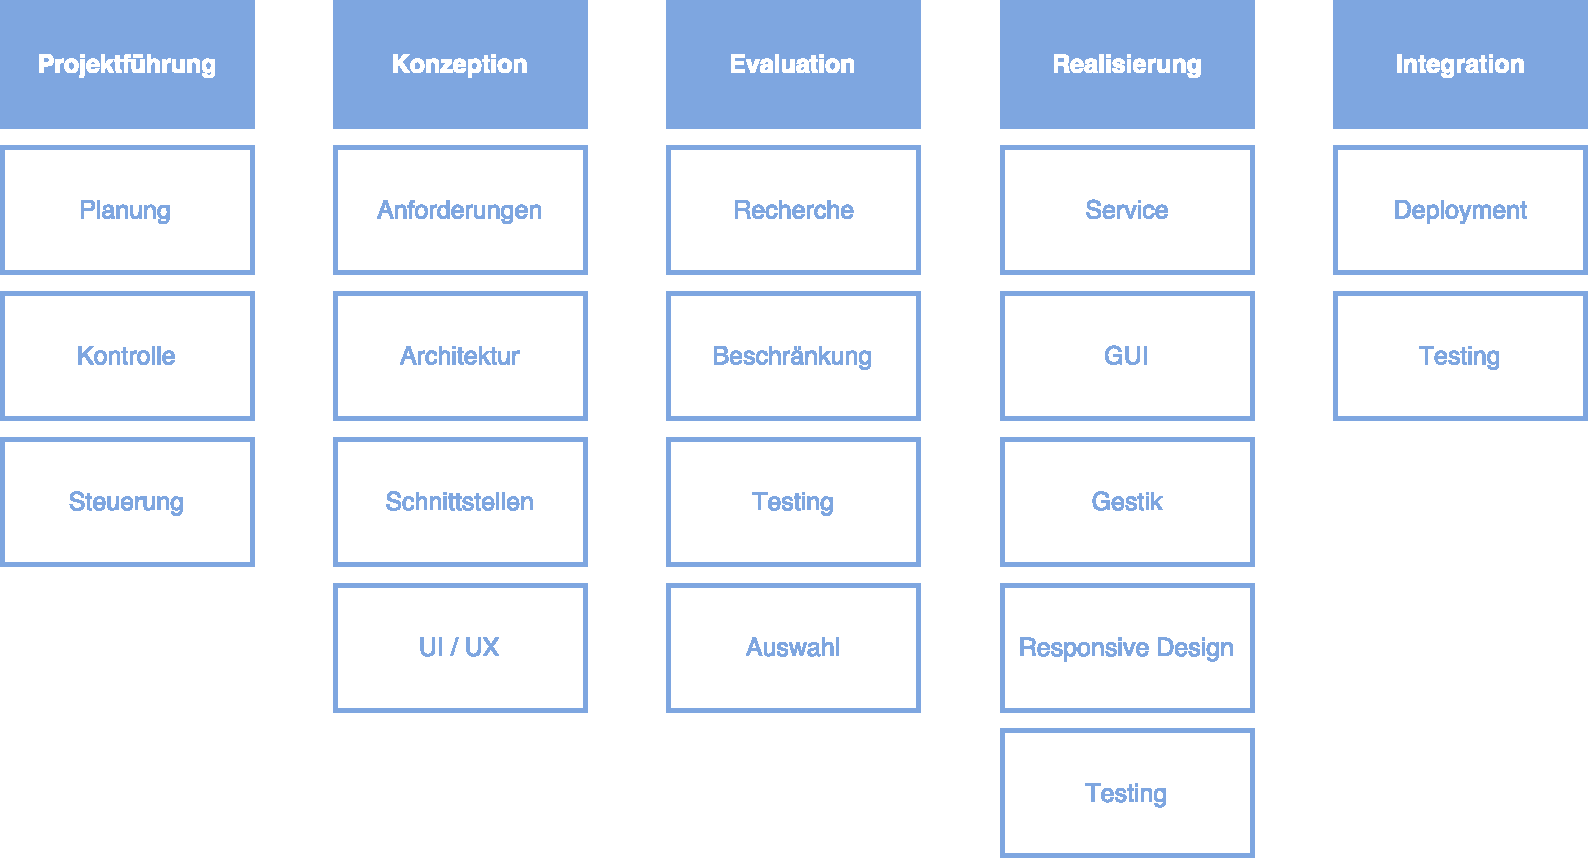
\includegraphics[width=1.5\textwidth]{Projektstrukturplan}
\caption{Projektstrukturplan}
\label{fig:projektstrukturplan}
\end{figure}
\end{landscape}

\newpage

\section{Rahmenplan}
Die Rahmenplanung, basierend auf der Projektstrukturplan (\autoref{fig:rahmenplan}), repräsentiert die zeitliche Planung des Projekts. Dabei werden Kalenderwochen anstelle von Daten oder Schulwochen verwendet. Dies kommt aufgrund des internationalen Rahmens, den damit verbundenen Zeitverschiebung und unterschiedlichen Stundenplänen. Enthalten sind alle Projektphasen, Sprints und Meilensteine, als auch alle Lieferobjekte welche im \autoref{lieferobjekte} weiter ausgeführt werden. Die Sprints haben absichtlich unterschiedliche Dauer, welche aufgrund der verschieden Projektphasen und deren Inhalt zugeordnet worden sind. Weiter werden administrative Elemente durch blaue Färbung und Entwicklungs-Elemente durch rote Färbung gekennzeichnet.

Eine grosse Rolle in der Rahmenplanung spielen die Meilensteine. Sie unterteilen das Projekt in Phasen, welche dadurch klar von einander getrennt sind. Ebenfalls sind sie eine wichtige Orientierungshilfe im Projekt und weisen den Weg damit das Projekt erfolgreich abgeschlossen werden kann. Die \autoref{tab:meilensteine} listet die Meilensteine auf.


\begin{longtable}{|p{1cm}|p{2cm}|p{8.5cm}|}
  \hline
    ID & Datum &  Beschreibung \\\hline
    M1 & 19.09.2016 & Administrativer Meilenstein, Kickoff\\\hline
    M2 & 10.10.2016 & Administrativer Meilenstein, Projektplanung abgeschlossen\\\hline
    M3 & 17.10.2016 & Entwicklung Meilenstein, Schnittstellen definiert\\\hline
    M4 & 07.11.2016 & Entwicklung Meilenstein, Evaluation Entscheid\\\hline
    M5 & 26.12.2016 & Entwicklung Meilenstein, Funktionale Oberfläche umgesetzt\\\hline
    M6 & 13.01.2017 & Entwicklung Meilenstein, Integration in \textbf{ikc-core} abgeschlossen\\\hline
    M7 & 20.01.2017 & Administrativer Meilenstein, 95\% erreicht\\\hline
    M8 & 31.01.2017 & Administrativer Meilenstein, PAWI Bericht Abgabe\\\hline
    M9 & 03.02.2017 & Administrativer Meilenstein, Präsentation\\\hline
    \caption{Meilensteine}
  \label{tab:meilensteine}
\end{longtable}

\improvement[inline]{Meilensteie jeweils auf Ende Woche setzen.}

\newpage

\begin{landscape}
\begin{figure}[ht]
\centering
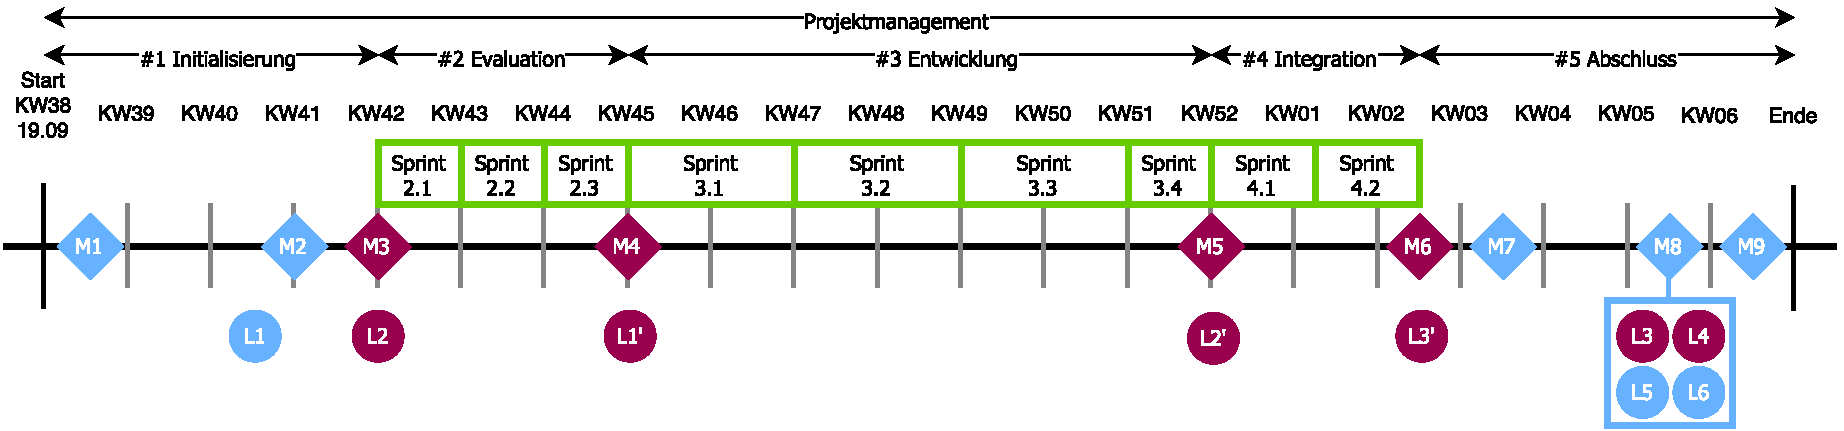
\includegraphics[width=1.7\textwidth]{Rahmenplan}
\caption{Rahmenplan}
\label{fig:rahmenplan}
\end{figure}
\end{landscape}

\newpage

\section{Projektziele} \label{projektziele}
Projektziele werden definiert, um den Projekterfolg an einigen möglichst konkreten Punkten zu messen. Diese sind in der folgenden \autoref{tab:projekt-ziele} aufgelistet.

\begin{longtable}{|p{1cm}  | p{10.5cm}|}
  \hline
    ID &  Beschreibung \\\hline
    Z1 & Ergänzung zur bestehenden Benutzeroberfläche.\\\hline
    Z2 & Entwicklung nach dem Konzept \textit{mobile first}.\\\hline
    Z3 & Intuitive, visuelle und effiziente Interaktion mit einem Netzwerk.\\\hline
    Z4 & Übersichtliche Visualisierung der \textit{Nodes} und \textit{Links}.\\\hline
    Z5 & Erweiterung der Funktionalität mittels Sichten (\textit{Views}).\\\hline
    \caption{Projektziele}
  \label{tab:projekt-ziele}
\end{longtable}

\section{Anforderungen} \label{anforderungen}

Für die weitere Unterteilung in Arbeitspakete und Stories werden die Anforderungen zunächst in Prosa gesammelt. Diese entstammen dem Kundenworkshop und der Aufgabenstellung und sind im Sinn der Projektziele (\autoref{projektziele}) ausgeführt. Die Anforderungen werden unterschieden in funktionale und nicht funktionale Anforderungen. Die funktionalen Anforderungen definieren direkt die Eigenschaften \autoref{tab:funktionale-anforderungen}. Nicht funktionale Anforderungen im Gegenteil definierten dabei die Leistung und die Randbedingungen, aufgelistet in \autoref{tab:nicht-funktionale-anforderungen}.

Die Priorisierung erfolgt nach dem MoSCoW-System:

\begin{longtable}{|p{1.5cm} | p{2.5cm} | p{7.2cm}|}
  \hline
    \# & Priorität & Beschreibung \\\hline
    M & Must Have & Bei dieser Anforderung handelt es sich um ein Muss, höchste Priorität.\\\hline
    S & Should Have & Diese Anforderung wird erwartet, normale Priorität.\\\hline
    C & Could Have & Tiefste Priorität, desiderata.\\\hline
    \caption{MosCow-Priorisierung}
    \footnote{\cite{moscow:hardvard}}
  \label{tab:moscow}
\end{longtable}


\begin{longtable}{|p{1.5cm} | p{1.5cm} | p{8.1cm}|}
  \hline
    ID & Priorität & Beschreibung \\\hline
    A1.1 & M & Die zugrunde liegende Datenbasis kann mittels eines Netzwerks visualisiert werden. Jenes besteht aus Knoten und Kanten, welche gerichtet und beschriftet sind. Sowohl Kanten als auch Knoten sind beschriftet.\\\hline
    A1.2 & M & Der zu erarbeitende Prototyp kann bidirektional mit dem \textit{ikc-core}-Prototypen interagieren. Änderungen am \textit{ikc-core} sind in der Visualisierung sichtbar. Es ist jedoch es auch möglich Änderungen direkt in der Visualisierung vorzunehmen.\\\hline
    A1.3 & S & Mittels der Visualisierung können die grundlegenden Datenbankoperationen \textit{CREATE}, \textit{READ}, \textit{UPDATE} und \textit{DELETE} (CRUD) teilweise direkt auf der Datenbasis des \textit{ikc-core} angewendet werden.\\\hline
    A1.3.1 & S & Es können sowohl Knoten aus dem Diagramm (View), als auch aus der Datenbasis (Model) gelöscht werden. Diese Vorgänge können klar unterschieden werden.\\\hline
    A1.3.2 & M & Knoten ohne Kanten können in der Visualisierung abgebildet werden.\\\hline
    A1.3.3 & M & Knoten können in der Visualisierung erstellt werden.\\\hline
    A1.4 & M & Der Prototyp kann auf Smartphones und Tablets benutzt werden.\\\hline
    A1.5 & S & Der Prototyp kann auf Laptops und Desktop-Computern benutzt werden.\\\hline    
    A1.6 & M & Mit Hilfe verschiedener Kriterien (beispielsweise Kontext oder Nachbarschaft) kann ein Teilnetzwerk visualisiert werden.\\\hline 
    A1.6.1 & S & Diese Teilgraphen (Sichten) können unabhängig von der Datenbasis persistiert werden. Es können, zusätzlich zu den Knoten und Kanten, auch deren relative Positionen in der Visualisierung gespeichert werden.\\\hline 
    A1.7 & C & Der Prototyp kann (unter anderem) mit Drag and Drop bedient werden.\\\hline
    A1.7.1 & S & Bidirektionale und unbeschriftete Verknüpfungen zwischen visualisierten Knoten können erstellt werden.\\\hline
    A1.7.2 & M & Ein, im bestehenden User-Interface, mittels der Suche gefundener Knoten kann direkt in die Visualisierung übernommen werden.\\\hline 
    A1.7.3 & S & Ein mittels der Suchfunktion gefundener Knoten kann auf einen bestehenden Knoten gezogen werden, um mit diesem eine Kante zu bilden.\\\hline 
    A1.7.4 & S & Knoten können innerhalb des Diagramms frei positioniert werden.\\\hline 
    A1.8 & M & Die Visualisierung kann innerhalb der bestehenden \textit{ikc-core} Oberfläche genutzt werden.\\\hline 
    A1.9 & S & In der Visualisierung könnnen auch Knoten mit mehr als sieben Kindknoten dargestellt werden: Sind mehr als sieben Kindknoten vorhanden, wird anstelle einer Repräsentation jedes einzelnen Knotens auf eine Liste gewechselt. Diese Liste kann zusätzlich mit einer Such- und oder Filterfunktion versehen werden.\\\hline  
    A1.10 & C & Die von einem Knoten aus- und eingehenden Kanten können auf- und zugeklappt (sichtbar-unsichtbar) werden.\\\hline
    A1.10.1 & C & Einzelne Kanten können individuell zugeklappt / ausgeblendet werden.\\\hline
     
    \caption{Funktionale Anforderungen}
  \label{tab:funktionale-anforderungen}
\end{longtable}

\begin{longtable}{|p{1.5cm} | p{1.5cm} | p{8.1cm}|}
  \hline
    ID & Priorität & Beschreibung \\\hline
    A2.1 & M & Bestehende Komponenten des \textit{ikc-core}, wo möglich, wiederverwendet bzw. erweitert (nachhaltige Entwicklung).\\\hline
    A2.2 & M & Die Visualisierung kann in verschiedenen Projekten wiederverwendet werden.\\\hline
    A2.3 & M & Die Visualisierung wird im \textit{ikc-core} integriert (Deployment).\\\hline
    A2.4 & M & Die Visualisierung wird parallel zum \textit{ikc-core} weiterentwickelt. Die Basis für die Visualisierung bildet ein Klon des bestehenden \textit{Repositories}. Ist die Entwicklung abgeschlossen, werden die beiden Entwicklungsstände mittels eines neuen \textit{Branches} \textit{zusammengeführt} werden.\\\hline
    A2.5 & M & Jegliche Daten werden auf der Dropbox des Benutzers persistiert.\\\hline
    A2.6 & S & Es wird eine intuitive, effiziente Bedienung angestrebt. Ein Mass für die Effizienz: $\frac{\text{Taps}}{\text{Task}}$\\\hline
    A2.7 & M & Randbedingungen 180h pro Person\\\hline
    A2.8 & S & Die Arbeit können in einem Arbeitsjournal, mindestens mit Angaben von Datum, Anzahl Stunden, Arbeitsschritt/Thema, nachverfolgt werden.\\\hline
    \caption{Nicht funktionale Anforderungen}
  \label{tab:nicht-funktionale-anforderungen}
\end{longtable}

\section{Risikoanalyse}\label{risikoanalyse}

In folgender Tabelle (\autoref{tab:risikoanalyse}) werden mögliche Risiken behandelt. Die Wahrscheinlichkeit ist mit P abgekürzt, R steht für Risiko und S für den Schaden, welcher mittels $P*R=S$ berechnet wird.


\begin{longtable}{|p{0.5cm} | p{7cm} | p{1cm}|  p{1cm}|  p{1cm}|}
  \hline
    ID & Beschreibung &  P & R & S \\\hline
    R1 & Wie in \autoref{subsec:international} bereits angesprochen wird das Projekt im \textbf{internationalen Rahmen} durchgeführt. Dies birgt einige Herausforderungen und bringt auch Riksiken mit sich: Die grösste Schwierigkeit bildet sicherlich die Zeitverschiebung. Aber auch die geographische Distanz und die lediglich im digitalen Rahmen gehaltenen Sitzungen sind nicht zu unterschätzen. Daher werden verschiedene Kommunikations-Tools angewendet, um dieser Problematik zu begegnen. & 1 & 3 & 3\\\hline
    R2 & Die Abgrenzung vom laufenden Projekt \textbf{\textit{IKC}} (vgl. \autoref{sec:scope}) ist klar festzulegen, damit es möglich wenig Überschneidungen und Unklarheiten gibt. Vollständige und detaillierte Arbeitsjournale, wie auch Protokolle bieten dabei wichtige Hilfestellung.  & 2 & 1 & 2\\\hline
    R3 & Die Zahl der Anforderungen ist verhältnismässig hoch. Im Rahmen der \textbf{360 zu leistenden Stunden} ist es wichtig sich nicht in Details oder Ausarbeitung jeglicher Finessen zu verlieren. Darum ist es umso wichtiger die Anforderungen klar zu priorisieren und auch entsprechend abzuarbeiten.  & 3 & 1 & 3\\\hline
    \caption{Risikoanalyse}
  \label{tab:risikoanalyse}
\end{longtable}

\section{Lieferobjekte}\label{lieferobjekte}

Neben den in der Aufgabenstellung vorgegebenen Lieferobjekte (\autoref{tab:set-lieferobjekte}) sind noch zusätzliche, interne Lieferobjekte (\autoref{tab:add-lieferobjekte}) festlegt. Diese sind lediglich als Unterstützung der Projektkontrolle, eine Art Orientierungshilfe, gedacht.

\begin{longtable}{|p{1cm} | p{2cm} | p{8.1cm}|}
  \hline
    ID & Datum &  Beschreibung \\\hline
    L1 & 30.09.2016 & Projektplanung.\\\hline
    L2 & 07.10.2016 & Anforderungskatalog.\\\hline
    L3 & 17.10.2016 & Lösungskonzept inkl. Schnittstellendefinition.\\\hline
    L4 & 31.01.2017 & Funktionale Software mit folgenden Eigenschaften:
    \begin{itemize}
        \item Integriert bestehenden Prototyp auf Basis React mit allen CRUD     Funktionen \& Schnittstellen zu Dropbox und Evernote
        \item Gibt die Möglichkeit zur visuellen Interaktion mit einem 
            (Teil-)Netzwerk: Knoten können per Drag \& Drop verknüpft werden
        \item Die Applikation läuft auf dem Mobile, Tablet, Laptop und Desktop (in     Priorität der Reihenfolge) $=>$ responsive CSS Template verwenden
    \end{itemize}
    \\\hline
    L5 & 31.01.2017 & Dokumentierter Source Code (für Methoden und Parameter).\\\hline
    L6 & 31.01.2017 & Benutzerhandbuch.\\\hline
    L7 & 31.01.2017 & PAWI-Bericht.\\\hline
    \caption{Vorgegebene Lieferobjekte}
  \label{tab:set-lieferobjekte}
\end{longtable}
 
\begin{longtable}{|p{1cm} | p{2cm} | p{8.1cm}|}
  \hline
    ID & Datum &  Beschreibung \\\hline
    L1' & 07.11.2016 & Abgeschlossene Evaluation der verschiedenen Frameworks zur Umsetzung der Visualisierung.\\\hline
    L2' & 26.12.2016 & Funktionale Visualisierung gemäss den funktionalen Anforderungen A1.3, A1.4, A1.5, A1.6, A1.7, A1.9 und A1.10. Bereit für die Integration in den \textit{ikc-core}.\\\hline
    L3' & 13.01.2017 & Abgeschlossene Integration der Visualisierung in den \textit{ikc-core} und Erfüllung aller Anforderungen insbesondere A1.1, A1.2.\\\hline
    \caption{Zusätzliche, interne Lieferobjekte}
  \label{tab:add-lieferobjekte}
\end{longtable}

%\section{Epics}



%\section{Stories}
